\chapter{System Architecture}
\label{ch:architecture}

\section{Guiding Principles}
\label{subsec:guiding_principles}

Tycho’s architecture is shaped by a small set of foundational principles that govern how measurements are interpreted, combined and ultimately attributed. These principles are architectural in nature: they articulate \emph{how} the system must reason about observations, not \emph{how} it is implemented. They establish the conceptual baseline that the subsequent sections refine in detail.

\begin{itemize}[leftmargin=1.2em]
    \item \textbf{Accuracy-first temporal coherence.}
    Architectural decisions prioritise the reconstruction of temporally coherent views of system behaviour. Observations are treated as samples of an underlying physical process, and the architecture is designed to preserve their temporal meaning rather than force periodic alignment.

    \item \textbf{Domain-aware interpretation.}
    Metric sources differ in semantics and cadence. The architecture respects these differences and avoids imposing artificial synchrony or uniform sampling behaviour across heterogeneous domains.

    \item \textbf{Transparency of assumptions.}
    All modelling assumptions must be explicit, inspectable and externally visible. The architecture prohibits implicit corrections or hidden inference steps that would obscure how measurements lead to attribution results.

    \item \textbf{Uncertainty as a first-class concept.}
    Missing, stale or delayed information is treated as uncertainty rather than error. Architectural components convey and preserve uncertainty so that later stages may interpret it correctly.

    \item \textbf{Separation of observation, timing and attribution.}
    Measurement collection, temporal interpretation and energy attribution form distinct architectural layers. This separation prevents cross-coupling, clarifies responsibilities and ensures that improvements in one layer do not implicitly alter the behaviour of others.
\end{itemize}

\section{Traceability to Requirements}
\label{subsec:req_traceability}

The architectural structure introduced in this chapter provides a direct response to the requirements established in \S~\ref{sec:conceptual_requirements}. Each requirement class corresponds to specific architectural mechanisms, ensuring that the system design follows from formal constraints rather than implementation convenience.

\textbf{Requirement: Temporal Coherence.}
Satisfied through event-time reconstruction, independent collector timelines, and window-based temporal alignment.

\textbf{Requirement: Domain-Level Consistency.}
Addressed by per-domain interpretation layers, domain-aware handling of metric semantics, and explicit decomposition of node-level signals.

\textbf{Requirement: Cross-Domain Reconciliation.}
Supported by a unified temporal model, window-level aggregation boundaries, and explicit reconciliation logic across domains during analysis.

\textbf{Requirement: Consistent Metric Interpretation.}
Ensured by separating observation from interpretation, enforcing stable metric semantics within each domain, and isolating heterogeneous metrics into dedicated processing paths.

\textbf{Requirement: Transparent Modelling Assumptions.}
Realised through explicit modelling steps, external visibility of assumptions, and separation between measured and inferred quantities.

\textbf{Requirement: Lifecycle-Robust Attribution.}
Enabled by metadata freshness guarantees, stable process–container mapping, and attribution rules that remain valid under workload churn.

\textbf{Requirement: Uncertainty-Aware Attribution.}
Supported by explicit treatment of stale or missing data, uncertainty propagation in window evaluation, and preservation of unexplained residuals.

\section{High-Level Architecture}
\label{sec:high_level_architecture}

\subsection{Subsystem Overview}
\label{subsec:subsystem_overview}

Tycho is organised into a small set of subsystems, each with a distinct responsibility. The following overview introduces these subsystems without yet describing their interactions.

\textbf{Timing engine.}
Defines the temporal reference used throughout the system and provides the notion of analysis windows. It is responsible for deciding when a window is complete and ready to be evaluated.

\textbf{Metric collectors.}
Acquire observations from hardware and software sources and attach timestamps in the global temporal reference. They expose their output as streams of samples without coordinating with each other.

\textbf{Metadata subsystem.}
Maintains the mapping between operating-system level entities and workload identities. It tracks relationships between processes, cgroups, containers and pods over time.

\textbf{Buffering and storage layer.}
Stores recent observations in bounded histories so that samples relevant to a given window can be retrieved efficiently. It treats metric streams and metadata as read-mostly records.

\textbf{Analysis engine.}
Interprets temporally aligned observations and metadata to produce energy estimates for each analysis window. It forms the logical bridge between measurement and attribution.

\textbf{Calibration framework.}
Derives auxiliary information about typical delays, update patterns and idle behaviour. It produces constraints and characterisations that other subsystems rely on for interpretation.

\textbf{Exporter.}
Exposes the results of the analysis engine to external monitoring systems as metrics ready for scraping and downstream processing.

\subsection{Dataflow and Control Flow}
\label{subsec:dataflow_control}

Before Tycho enters normal operation, external calibration scripts determine approximate delay characteristics for all relevant metric sources. At startup, Tycho’s internal calibration component derives suitable polling frequencies for metric collectors and metadata acquisition, providing the initial operating parameters for the system.

During runtime, control flow originates in the timing engine. It triggers each collector according to its calibrated polling frequency, but collectors operate independently: they sample their respective domains without synchronising with each other, and each sample is appended to the appropriate buffer together with its timestamp and quality indicators. In parallel, metadata acquisition proceeds on its own schedule, refreshing the mappings between processes, cgroups and workload identities in the metadata cache.

The timing engine also governs when analysis occurs. At regular intervals—constituting fixed-length analysis windows—it initiates a new evaluation cycle irrespective of how many samples have been collected. Each cycle begins by estimating idle behaviour for the relevant hardware domains based on the buffered observations. The analysis engine then interprets the buffered metric samples, the metadata cache and the idle characterisations, taking calibrated delays into account when reconstructing the temporal structure of the window. It produces per-window energy estimates for all domains and workloads.

Once analysis completes, the exporter publishes the resulting metrics in a form suitable for ingestion by external monitoring systems. Calibration remains active in the background throughout the system’s lifetime: it observes collector behaviour and derived quantities over longer time spans and refines its characterisations when needed, informing both the timing and analysis components without altering any collected data.

\begin{figure}[H]
    \centering
    \includegraphics[width=0.9\textwidth]{Figures/drawio/tycho_architecture_high.png}
    \caption[Subsystem Architecure, Dataflow and Control Flow]{Subsystem Architecure, Dataflow and Control Flow}
    \label{vt1_fig:tycho_architecture_high}
\end{figure}

\section{Temporal Model and Timing Engine}
\label{sec:timing_engine}

Tycho’s temporal architecture provides a coherent framework for relating heterogeneous metric streams to fixed-duration analysis windows. It establishes a common time base, defines how collectors operate, and specifies how windows are formed and interpreted. The model is intentionally simple: collectors run independently, timestamps reflect poll time, and all temporal reasoning occurs during analysis.

% ----------------------------------------------------------------------
\subsection{Event-Time Model and Timestamp Semantics}
\label{subsec:event_time}

Tycho adopts a single monotonic time base for all temporal coordination. Collectors timestamp each sample at the moment of observation; these timestamps reflect poll time, not the physical instant at which the underlying hardware event occurred. Event time is therefore a modelling construct used by the analysis engine when interpreting delay, freshness and update behaviour.

This separation keeps collectors lightweight and domain-agnostic. Each collector reports only what it directly observes; the analysis engine later interprets these timestamps in context, using calibration-derived delay characteristics to approximate underlying temporal structure.
% ----------------------------------------------------------------------
\subsection{Independent Collector Schedules}
\label{subsec:independent_timelines}

Tycho employs independent, domain-aware sampling schedules. During startup the timing engine configures one schedule per collector, after which each collector operates autonomously on its own periodic trigger. No global poll loop exists and collectors do not synchronise with one another. They push samples only when a new observation is available.

This decoupling avoids artificial temporal alignment and preserves each domain’s intrinsic update behaviour. Collector timestamps are placed directly on the global monotonic time axis, allowing later reconstruction without imposing shared cadence or shared sampling semantics.

% ----------------------------------------------------------------------
\subsection{Window Construction and Analysis Triggering}
\label{subsec:window_construction}

Analysis proceeds in fixed-duration windows defined solely by periodic triggers from the timing engine. If the triggers occur at monotonic times \(T_0, T_1, T_2, \dots\), window \(W_i\) is the half-open interval \([T_i, T_{i+1})\). Window duration is nominally constant but may drift slightly, which is acceptable for attribution.

When a window closes, the analysis engine performs two conceptual phases:

\begin{enumerate}[label=(\roman*)]
\item \emph{idle characterisation}, using long-term buffered history across all relevant domains, and  
\item \emph{window reconstruction and attribution}, using all samples whose timestamps precede \(T_{i+1}\).
\end{enumerate}

Only energy for the current window is attributed and exported, but additional historical samples inform delay interpretation, idle estimation and interpolation.

Tycho treats domains asymmetrically: CPU and software metrics are always required; GPU and Redfish domains contribute when available. Samples too old to fall within the current window do not contribute directly but may still inform background characterisation. Windows remain valid when optional domains are absent.

A sample is considered stale relative to a window when its poll timestamp predates \(T_i\) by more than a domain-specific tolerance. Stale samples are ignored for direct reconstruction but do not invalidate the window.

\begin{figure}[H]
    \centering

    % Define custom color
    \definecolor{windowblue}{HTML}{BDC6FF}
    \colorlet{windowblueA}{windowblue!40}

    \begin{tikzpicture}[
        >=Stealth,
        scale=1,
        every node/.style={font=\small}
    ]

    % Time axis
    \draw[->] (0,0) -- (11,0) node[anchor=west] {time};

    % Window boundaries
    \draw[very thick] (3,0.2) -- (3,-0.2);
    \draw[very thick] (8,0.2) -- (8,-0.2);
    \node[below] at (3,-0.2) {$T_i$};
    \node[below] at (8,-0.2) {$T_{i+1}$};

    % Window highlight with your color
    \draw[fill=windowblueA, draw=none] (3,0.3) rectangle (8,4.1);
    \node[below] at (5.5,4.1) {Window $W_i = [T_i, T_{i+1})$};

    % Collector lines
    \node[left] at (0,1) {Collector C};
    \draw (0,1) -- (10.5,1);

    \node[left] at (0,2) {Collector B};
    \draw (0,2) -- (10.5,2);

    \node[left] at (0,3) {Collector A};
    \draw (0,3) -- (10.5,3);

    % Samples for A
    \foreach \x/\style in {1/gray, 3.5/black, 6.2/black, 9/gray} {
        \draw[thick,\style] (\x,0.8) -- (\x,1.2);
    }

    % Samples for B
    \foreach \x/\style in {2.5/gray, 3.2/black, 4.1/black, 7.9/black, 9.5/gray} {
        \draw[thick,\style] (\x,1.8) -- (\x,2.2);
    }

    % Samples for C
    \foreach \x/\style in {2/gray, 5.0/black, 8.5/gray} {
        \draw[thick,\style] (\x,2.8) -- (\x,3.2);
    }

    \node[gray] at (1.0,0.4) {outside window};
    \node[gray] at (9.3,0.4) {outside window};

    \end{tikzpicture}

    \caption{Analysis window $W_i$ in relation to collectors}
    \label{fig:window_alignment}
\end{figure}


\subsection{Comparison to Kepler Timing Model}
\label{subsec:kepler_comparison}

Kepler employs a synchronous timing model in which all metric domains (except Redfish) are sampled within a single periodic poll cycle (default: 3 seconds). This fixed-length interval defines both the sampling cadence and the logical unit of attribution. Redfish updates occur at a much slower rate (default: 60 seconds), and the most recent Redfish value is reused across multiple attribution intervals. Export occurs on a separate cadence, which may not align with the attribution window.

Tycho diverges fundamentally: collectors run independently, analysis windows are defined by attribution triggers rather than poll cycles, heterogeneous update patterns are supported natively, and export occurs immediately after each attribution step. This structure enables finer temporal resolution, avoids dependence on synchronous polling behaviour, and eliminates inconsistencies between data collection and publishing intervals.

Figures~\ref{vt1_fig:tycho_timingDiagram} and \ref{vt1_fig:kepler_timingDiagram} illustrate the respective timing behaviour of Tycho and Kepler, highlighting their polling patterns, sampling semantics and analysis-window alignment. Figures~\ref{vt1_fig:tycho_timingDiagram_high} and \ref{vt1_fig:kepler_timingDiagram_high} provide a higher-level view to show the Prometheus export behaviour more clearly.

\begin{figure}[H]
    \centering
    \begin{subfigure}{1\textwidth}
        \includegraphics[width=\textwidth]{Figures/drawio/tycho_timingDiagram.png}
        \caption{Tycho Timing Model}
        \label{vt1_fig:tycho_timingDiagram}
    \end{subfigure}
    \begin{subfigure}{1\textwidth}
        \includegraphics[width=\textwidth]{Figures/drawio/kepler_timingDiagram.png}
        \caption{Kepler Timing Model}
        \label{vt1_fig:kepler_timingDiagram}
    \end{subfigure}
    \caption[Comparison between Tycho and KeplerTiming Model]{Comparison: Tycho and Kepler Timing Model}
\end{figure}

\begin{figure}[H]
    \centering
    \begin{subfigure}{0.85\textwidth}
        \includegraphics[width=\textwidth]{Figures/drawio/tycho_timingDiagram_high.png}
        \caption{Tycho Prometheus Export Timing Model}
        \label{vt1_fig:tycho_timingDiagram_high}
    \end{subfigure}
        \begin{subfigure}{0.85\textwidth}
        \includegraphics[width=\textwidth]{Figures/drawio/kepler_timingDiagram_high.png}
        \caption{Kepler Prometheus Export Timing Model}
        \label{vt1_fig:kepler_timingDiagram_high}
    \end{subfigure}
    \caption[Comparison between Tycho and Kepler export behaviour]{Comparison: Tycho and Kepler export behaviour}
\end{figure}




% ----------------------------------------------------------------------

\section{Metric Sources as Temporal Actors}
\label{sec:metric_sources}

\subsection{eBPF and Software Counters}
\label{subsec:ebpf_temporal}

The eBPF and software counter domain represents Tycho’s event-driven view of CPU
activity.  
Unlike hardware domains that report values at fixed sampling times, this domain
emits utilisation information at the moment execution state changes occur.  
These events form a temporally dense and workload-dependent signal that describes
how processor time is distributed across user tasks, kernel execution, interrupt
handling, and idle periods.  
All higher-level aggregation is performed in userspace and is decoupled from the
event timing itself.

The domain contributes three classes of metrics with distinct temporal semantics.
\begin{itemize}
    \item \emph{Event-driven metrics} capture transitions in processor ownership.
    They record the exact time at which execution begins or ends for a given
    context and therefore define precise temporal boundaries for attribution
    windows.
    \item \emph{Cumulative counters} accumulate activity or duration over time and
    expose their values when queried.  
    Their effective resolution is determined by the polling interval rather than
    by internal update frequency.
    \item \emph{Quasi-instantaneous counters} sample hardware performance state at
    activity boundaries.  
    Although observed at discrete points, their semantics remain tied to the
    execution periods they describe.
\end{itemize}

Two architectural properties follow directly from this structure.  
First, event-driven updates introduce no domain delay and therefore require no
delay calibration.  
Second, the collector may operate at an arbitrary polling cadence, since temporal
alignment is guaranteed by the event timestamps themselves.  
In Tycho the default interval is chosen to align with the RAPL window for
convenience rather than correctness.  
Each event also carries the current container context, ensuring correct
attribution when workloads migrate across control groups.

Within Tycho’s temporal model, this domain occupies a special role.  
It accumulates fine-grained ownership information at execution boundaries and
exposes it at analysis windows without influencing their timing.  
The resulting signals form a complete temporal partition of CPU activity within
each interval, supporting proportional attribution and reducing uncertainty in
downstream energy modelling.  
Architecturally, the eBPF domain therefore provides the most precise and
temporally coherent view of processor utilisation available to the system.

\subsection{RAPL Domains}
\label{subsec:rapl_temporal}

RAPL exposes cumulative energy counters for a set of logical CPU-related domains,
including package, cores, uncore, and memory.  
Each domain provides a monotonically increasing counter that reflects total energy
consumed since a hardware-defined reference point.  
These counters advance independently of Tycho’s sampling schedule and describe
the continuous energy behaviour of the processor.

Within Tycho, RAPL counters are observed at fixed tick boundaries.  
At each tick the current counter values are recorded, and interval energy follows
from the difference between consecutive readings.  
RAPL therefore contributes energy over time rather than instantaneous power, with
temporal resolution defined entirely by the tick interval.  
Because hardware updates occur at a much higher rate than sampling, the counters
behave as effectively continuous at the chosen time scale.

RAPL sampling is synchronised with Tycho’s timing engine so that each interval
contains exactly one cumulative reading per domain.  
No delay calibration is required: internal update behaviour is already integrated
into the counters and does not affect interval attribution.  
Architecturally, RAPL acts as a stable and low-noise source of CPU-adjacent energy.

The domain structure of RAPL aligns naturally with Tycho’s requirement for
domain-level consistency.  
Per-socket counters for package, core, uncore, and memory domains form a coherent
and stable decomposition of CPU energy that is preserved across intervals.  
This decomposition provides a reliable baseline against which software-side
utilisation signals can be related during attribution.

\subsection{Redfish/BMC Power Source}
\label{subsec:redfish_temporal}

Redfish provides an out-of-band view of total node power through the server’s
Baseboard Management Controller.  
Unlike in-band sources such as RAPL or eBPF telemetry, Redfish publishes
instantaneous power values at coarse and irregular intervals determined entirely
by the BMC implementation.  
These updates are asynchronous with respect to Tycho’s timing engine and cannot
be controlled or accelerated by the system.

Within Tycho’s architecture, Redfish is therefore treated as a \emph{latently
published external observation} rather than a synchronisable metric source.
Sampling is performed at fixed tick boundaries using the global monotonic
timebase, but the temporal authority remains with the BMC.  
Repeated values are common, and new measurements may appear only after several
ticks.  
Redfish thus does not define time; it constrains it.

To make this uncertainty explicit, each Redfish observation is annotated with a
\emph{freshness} value that expresses the temporal distance between the BMC’s
reported update time, when available, and Tycho’s collection time.  
Freshness is an architectural quality indicator rather than a correction
mechanism.  
It allows downstream analysis to reason about the temporal reliability of each
reading without assuming regular publication or low latency.

The irregular nature of Redfish publication also requires continuity guarantees.
When no new BMC update appears for an extended period, Tycho emits an explicit
continuation of the last known power value.  
Continuation samples preserve a complete and chronologically consistent power
timeline while making the absence of new information explicit.  
They carry the same timestamping and freshness semantics as true updates but do
not indicate new power measurements.

Despite its limited temporal resolution, Redfish serves as Tycho’s authoritative
source for total node power.  
Its measurements provide a stable reference against which CPU- and
accelerator-level energy estimates can be interpreted.  
Architecturally, Redfish complements fine-grained in-band domains by anchoring
the system’s global energy view, while its coarse and irregular behaviour is
accommodated through explicit timestamping, freshness annotation, and controlled
continuation rather than through high-frequency sampling or delay correction.

\subsection{GPU Collector Architecture}
\label{subsec:gpu_architecture}

Accelerators form a significant share of the power consumption of modern compute
nodes.  Tycho therefore integrates GPU telemetry into the same unified temporal
framework that governs RAPL, Redfish, and eBPF sources.  NVIDIA devices expose
energy-relevant information only at discrete publish moments inside the driver,
so GPU sampling cannot rely on periodic polling alone.  Instead, Tycho aligns
sampling with the device's internal update behaviour and publishes at most one
\code{GpuTick} for each confirmed hardware update.  All GPU ticks share the
global monotonic timebase that underpins Tycho's event-time model
(\S~\ref{sec:tycho_timing_engine}).

\paragraph{Architectural Role}
The GPU subsystem provides two forms of telemetry.  
Device-level metrics describe the instantaneous operating state of each
accelerator, including power, utilisation, memory, thermals, and clock data.
Process-level metrics describe backend-aggregated utilisation over a defined
wall-clock window.  Both streams are combined into a single \code{GpuTick} that
represents the accelerator state at a specific moment in Tycho's global
timeline.  GPUs and MIG instances are treated as independent logical devices.

A central architectural design choice is the use of high-frequency
\emph{instantaneous} power fields exposed through NVIDIA’s field interfaces,
rather than relying exclusively on the conventional averaged power signal.
Most existing GPU energy analyses depend on the one-second trailing average
returned by \code{nvmlDeviceGetPowerUsage}, which obscures short-lived changes in
power demand.
By incorporating instantaneous power samples alongside averaged values, Tycho
preserves substantially richer temporal structure at the telemetry source
itself.
This additional signal fidelity is a prerequisite for sub-second attribution
and is later exploited by the analysis engine to improve temporal accuracy.

\paragraph{Backend Abstraction}
The GPU collector interfaces with NVIDIA hardware through \code{NVML}, which
provides access to device-level and process-level telemetry.
The architecture introduces a backend abstraction layer to decouple the
collector from a specific vendor interface.
This abstraction permits alternative backends, such as \code{DCGM}, to be
integrated in the future without altering the surrounding timing and buffering
logic. In the current system, \code{NVML} is the sole implemented backend.

The architecture does not assume uniform telemetry availability across devices.
Cumulative energy counters, instantaneous power fields, and process-level
utilisation may or may not be exposed depending on GPU generation and
configuration.
These capability differences are treated as properties of individual devices
and handled through per-device feature masks within the implementation.

\paragraph{Conceptual Sampling Model}
GPU drivers update power and utilisation metrics at discrete, hardware-defined
cadences that are not visible to callers.  Polling at a fixed interval is fundamentally mismatched to this behaviour.
If the polling frequency is lower than the internal publish cadence, updates are
missed; if it is higher, the collector repeatedly observes identical values.
Over time, this mismatch leads to aliasing, redundant samples, and temporal drift
relative to other metric sources.

The sampling model distinguishes two conceptual modes.  
In base mode, the subsystem polls at a moderate frequency to track slow drift in
the device's cadence.  
In \emph{phase-aware sampling} mode, the subsystem temporarily increases its sampling frequency when
Tycho's timebase approaches a predicted publish moment.  This concentrates
sampling effort where a fresh update is expected and reduces latency between the
hardware update and Tycho's observation of it. As a result, a new sample can be dected earlier (and hence, with a more accurate timestamp), while avoiding additional overhead introduced by constant hyperpolling.
The architecture guarantees that sampling remains event-driven rather than periodic.

Figure~\ref{fig:gpu_phaseaware_timeline} illustrates this behaviour at the
architectural level, showing the relationship between the GPU’s implicit publish
events, Tycho’s adaptive polling activity, and the resulting sequence of emitted
\code{GpuTick}s.

\begin{figure}[H]
\centering
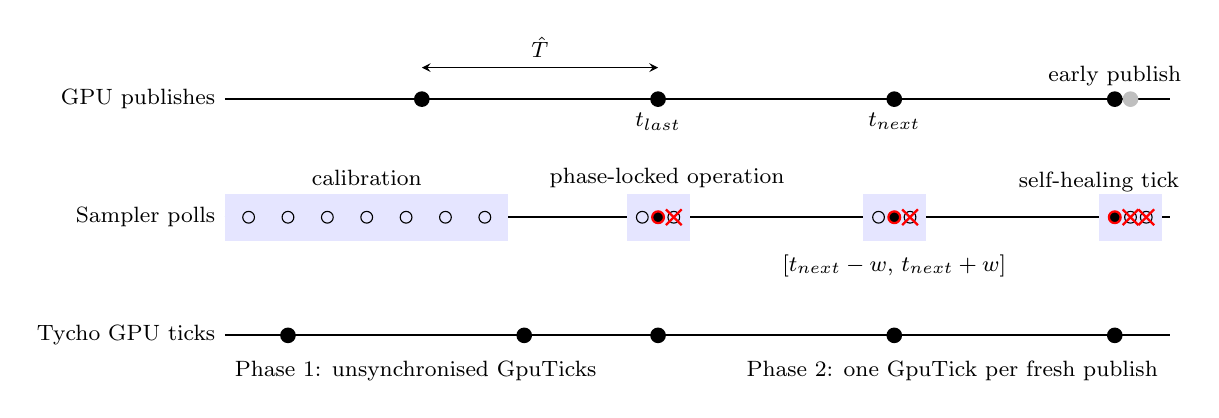
\begin{tikzpicture}[
    >=stealth,
    publish/.style={circle,fill=black,inner sep=2pt},
    poll-calib/.style={circle,draw=black,inner sep=1.5pt},
    poll-base/.style={circle,fill=black,inner sep=1.5pt},
    poll-burst/.style={circle,draw=black,inner sep=1.5pt},
    tick/.style={circle,fill=black,inner sep=2pt},
    timeline/.style={thick},
    label/.style={font=\footnotesize}
]

% Horizontal extents
\def\xmin{0}
\def\xmax{12}

% Y positions for the three lanes
\def\ygpu{3.2}
\def\ysampler{1.7}
\def\ytick{0.2}

% ------------------------------------------------------------------
% 1) GPU publish lane (ground truth)
% ------------------------------------------------------------------
\draw[timeline] (\xmin,\ygpu) -- (\xmax,\ygpu);
\node[label,anchor=east] at (\xmin,\ygpu) {GPU publishes};

% True publish events (roughly equidistant), last one early at 11.3
\foreach \x in {2.5,5.5,8.5} {
  \node[publish] at (\x,\ygpu) {};
}

% Actual early publish
\node[publish] at (11.3,\ygpu) {};
\node[label,anchor=south] at (11.3,\ygpu+0.05) {early publish};

% Expected publish (ghost marker) at 11.5
\node[circle,fill=gray!50,inner sep=2pt] at (11.5,\ygpu) {};

% Annotate approximate period between two publishes
\draw[<->] (2.5,\ygpu+0.4) --
    node[label,above] {$\hat{T}$}
    (5.5,\ygpu+0.4);

% Mark t_last and t_next for illustration
\node[label,anchor=north] at (5.5,\ygpu-0.05) {$t_{\text{last}}$};
\node[label,anchor=north] at (8.5,\ygpu-0.05) {$t_{\text{next}}$};

% ------------------------------------------------------------------
% 2) Sampler lane (calibration + phase-locked polls with burst window)
% ------------------------------------------------------------------
\draw[timeline] (\xmin,\ysampler) -- (\xmax,\ysampler);
\node[label,anchor=east] at (\xmin,\ysampler) {Sampler polls};

% Calibration phase block (left)
\def\xcalibStart{0.0}
\def\xcalibEnd{3.6}
\fill[blue!10] (\xcalibStart,\ysampler-0.3) rectangle (\xcalibEnd,\ysampler+0.3);
\node[label] at ({0.5*(\xcalibStart+\xcalibEnd)},\ysampler+0.50) {calibration};

% Calibration-phase polls (irregular, more frequent)
\foreach \x in {0.3,0.8,1.3,1.8,2.3,2.8,3.3} {
  \node[poll-calib] at (\x,\ysampler) {};
}

% Burst-style windows around predicted publish times in phase-locked regime
\def\tpred{5.5}
\def\whalf{0.4}
\fill[blue!10] (\tpred-\whalf,\ysampler-0.3) rectangle (\tpred+\whalf,\ysampler+0.3);

\def\tpred{8.5}
\def\whalf{0.4}
\fill[blue!10] (\tpred-\whalf,\ysampler-0.3) rectangle (\tpred+\whalf,\ysampler+0.3);
\node[label,anchor=north] at (\tpred,\ysampler-0.35)
  {$[t_{\text{next}}-w,\,t_{\text{next}}+w]$};

\def\tpred{11.5}
\def\whalf{0.4}
\fill[blue!10] (\tpred-\whalf,\ysampler-0.3) rectangle (\tpred+\whalf,\ysampler+0.3);

% Phase-locked base polls: successful observation polls
\node[poll-base,draw=red,thick] at (5.5,\ysampler) {};
\node[poll-base,draw=red,thick] at (8.5,\ysampler) {};
% Last window: successful observation comes slightly early
\node[poll-base,draw=red,thick] at (11.3,\ysampler) {};
\node[label,anchor=south] at (11.1,\ysampler+0.2) {self-healing tick};

% Additional burst-mode polls around t_next (denser sampling inside window)
\foreach \x in {5.3,5.7,8.3,8.7,11.5,11.7} {
  \node[poll-burst] at (\x,\ysampler) {};
}

% Polls that get skipped AFTER a successful observation:
% - in the first two windows: the late burst poll
% - in the last window: the scheduled base poll at 11.5 and the late burst poll at 11.7
\foreach \x in {5.7,8.7,11.5,11.7} {
  \draw[red,thick] (\x-0.10,\ysampler-0.10) -- (\x+0.10,\ysampler+0.10);
  \draw[red,thick] (\x-0.10,\ysampler+0.10) -- (\x+0.10,\ysampler-0.10);
}

% Optional annotation: phase-locked region
\node[label,anchor=west] at (4.0,\ysampler+0.50) {phase-locked operation};

% ------------------------------------------------------------------
% 3) Tycho GPU tick lane (two phases)
% ------------------------------------------------------------------
\draw[timeline] (\xmin,\ytick) -- (\xmax,\ytick);
\node[label,anchor=east] at (\xmin,\ytick) {Tycho GPU ticks};

% Phase 1: same cadence as publishes, but not phase-aligned (during calibration)
\foreach \x in {0.8,3.8} {
  \node[tick] at (\x,\ytick) {};
}

% Phase 2: phase-locked, one tick per fresh device update
\foreach \x in {5.5,8.5,11.3} {
  \node[tick] at (\x,\ytick) {};
}

\node[label,anchor=west] at (0.0,\ytick-0.45)
  {Phase 1: unsynchronised \code{GpuTick}s};

\node[label,anchor=west] at (6.5,\ytick-0.45)
  {Phase 2: one \code{GpuTick} per fresh publish};

\end{tikzpicture}
\caption{Phase-aware GPU polling timeline}
\label{fig:gpu_phaseaware_timeline}
\end{figure}

\paragraph{Tick Semantics}
A \code{GpuTick} is emitted only when Tycho detects a genuinely new hardware
update.  Each tick contains a snapshot of device-level metrics and, when
available, process-level utilisation aligned to the same monotonic timestamp.
This design ensures that GPU measurements participate in Tycho's
cross-domain correlation without interpolation, resampling, or ad hoc
realignment.  The one-to-one correspondence between hardware updates and GPU
ticks is a core architectural guarantee and the primary distinction between
Tycho's approach and traditional periodic sampling. This guarantee is visually summarised in Figure~\ref{fig:gpu_phaseaware_timeline}.

\paragraph{Process Telemetry Integration.}
Process-level metrics describe aggregated utilisation over a wall-clock window
that is defined by the backend rather than Tycho's timing engine.  The
architecture treats these windows as retrospective measurements that must be
aligned with the device timeline.  Each process record is anchored to the
timestamp of the device snapshot that triggered its acquisition.  This preserves
temporal coherence in spite of the retrospective semantics of process telemetry
and supports multi-tenant attribution across GPU workloads.

\paragraph{Integration with the Global Timing Model}
All GPU ticks are timestamped using Tycho's global monotonic timebase and
inserted into the multi-domain ring buffer
(\S~\ref{subsec:ringbuffer_overview}).  This ensures strict temporal ordering
relative to RAPL, Redfish, and eBPF data.  The architecture maintains the
principle of domain autonomy: each subsystem generates updates according to its
own temporal behaviour, while the analysis engine later fuses these streams into
a consistent attribution result.

\paragraph{Architectural Limitations}
Although the architecture abstracts over backend differences, several structural
constraints remain. Telemetry capabilities vary significantly across NVIDIA devices and driver
configurations.
Some accelerators expose high-quality instantaneous power fields and cumulative
energy counters, while others provide only averaged power and coarse utilisation.

The implicit publish cadence may drift under DVFS or thermal transitions, which
limits the predictability of update edges.  
Tycho mitigates these effects through robust sampling logic in the implementation,
but the fidelity of the resulting GPU timeline remains bounded by the behaviour
of the underlying hardware.

Overall, the GPU subsystem elevates accelerator telemetry to a first-class
component of Tycho's energy model.  By aligning sampling with the device's
publish behaviour and unifying device and process metrics under a single
timestamping model, the architecture enables precise, temporally consistent
attribution in heterogeneous accelerator environments.

\section{Metadata Collection Subsystem}
\label{sec:arch_metadata_collection}

Tycho treats workload identity as a first-class architectural concern that is
strictly separated from numerical telemetry.
While energy and utilisation collectors emit temporally ordered measurement
streams, metadata captures the structural relationships required to interpret
those streams during analysis.
This includes the association of processes, containers, and pods as they evolve
over the lifetime of a node.

Metadata is maintained as cached identity state rather than as a time series.
It is neither aggregated nor iterated over analysis windows and does not
participate directly in temporal correlation.
Instead, metadata provides a bounded, continuously refreshed snapshot of recent
workload structure that must remain sufficiently fresh and temporally consistent
to support later attribution.
Consequently, metadata collection prioritises controlled refresh and bounded
lifetime over high-frequency or event-level precision.

\paragraph{Subsystem overview.}
The metadata subsystem forms a dedicated architectural layer that operates
independently of metric collection and analysis.
It consists of a small set of autonomous collectors coordinated through a single
metadata controller, which constitutes the sole authority over metadata mutation
and lifecycle management.
Collectors observe the system independently, but all state updates are mediated
by the controller, enforcing a clear separation between identity acquisition and
subsequent analytical processing.

\paragraph{Dual-collector model.}
Workload identity is inherently multi-sourced.
Tycho therefore integrates two complementary metadata collectors, each providing
a partial and independently valid view of system state:
\begin{itemize}
  \item \textbf{proc-collector:} observes process identity, execution context, and
        cgroup membership directly from the Linux kernel via the filesystem
        interface, providing authoritative runtime state independent of
        orchestration abstractions.
  \item \textbf{kubelet-collector:} acquires pod- and container-level identity from
        the Kubernetes node agent, exposing scheduling and lifecycle information
        unavailable at the operating-system level.
\end{itemize}
The metadata subsystem does not attempt to fuse or interpret these views at
collection time.
Instead, it records the most recent identity state observed by each source and
defers reconciliation to analysis-time logic.

\paragraph{Controller-based coordination and scheduling.}
Metadata collection in Tycho is explicitly \emph{analysis-driven}.
The start of an analysis cycle constitutes the primary trigger for metadata
refresh and is treated as the highest-priority collection opportunity.
When an analysis window begins, the analysis engine requests a best-effort
refresh of all registered metadata collectors in order to obtain the most recent
possible identity state.

Autonomous metadata collectors exist as a secondary mechanism whose sole purpose
is to bound metadata age when analysis intervals are long.
These collectors execute under controller supervision and are explicitly
subjugated to analysis-driven collection.
If an analysis-triggered refresh is imminent, periodic collectors are suppressed
and defer execution to the analysis engine, preventing redundant collection in
short succession.

All collectors register with a central metadata controller, which arbitrates
between analysis-triggered and background execution.
The controller tracks the timestamp of the most recent successful observation for
each collector and enforces source-specific freshness constraints.
Collection is permitted only when required to satisfy source-specific freshness
constraints. As a result, metadata may be refreshed multiple times within a single analysis
window under long-running analysis, while redundant collection near analysis
boundaries is suppressed to reduce overhead.

This prioritisation establishes a clear architectural guarantee.
Metadata is maximally fresh at analysis start, redundant collection is avoided,
and collection overhead remains bounded independently of both analysis frequency
and global scheduling cadence.


\paragraph{Metadata state and lifetime model.}
Collected metadata is stored in a dedicated in-memory state that represents a
bounded snapshot of recent workload identity.
Unlike the ring-buffer–based design used for metric data, the metadata store
retains only the most recent valid representation of each observed entity.
Entries correspond to identity-bearing objects such as processes, containers, and
pods and are keyed by stable identifiers.
New observations update entries in place; historical versions and event sequences
are not preserved.

Each metadata entry carries a monotonic timestamp anchored to Tycho’s global
timebase, allowing identity state to be interpreted consistently alongside energy
and utilisation measurements.
Metadata is considered valid from its most recent observation until it is removed
by lifecycle management.
Garbage collection is horizon-based and enforced exclusively by the controller,
which removes entries once they fall outside the retained temporal window.
Collectors never delete metadata directly, ensuring deterministic expiry and
consistent memory bounds.

By coupling metadata lifetime to a bounded horizon rather than to explicit
lifecycle events, the subsystem remains robust to incomplete or delayed
observations.
Terminated processes, containers, and pods persist only long enough to support
overlapping analysis windows and are removed automatically thereafter.

\section{Calibration}
\label{sec:calibration}

Calibration is an auxiliary architectural subsystem that bounds temporal
uncertainty introduced by hardware-controlled metric publication.
It exists to constrain polling behaviour and temporal alignment for metric
sources whose update cadence or observable reaction latency is externally
governed and not analytically predictable.
Calibration is applied selectively and only where such uncertainty significantly
affects the correctness of subsequent analysis.

Calibration produces static, conservative parameters that are consumed by the
timing and analysis subsystems.
It does not participate in runtime attribution, does not adapt dynamically, and
does not operate on live metric streams.
By resolving temporal uncertainty ahead of time, calibration allows the runtime
system to remain deterministic, bounded, and non-intrusive.

Tycho distinguishes two independent calibration concerns:
\emph{polling-frequency calibration}, which bounds how often a metric source must
be queried to avoid undersampling hardware updates, and \emph{delay calibration},
which bounds the latency between a workload transition and the first observable
reaction in a metric stream.
These concerns are orthogonal and are applied only where their respective
assumptions hold.

\paragraph{Polling-frequency calibration.}
Polling-frequency calibration applies to metric sources whose publish cadence is
hardware-controlled and approximately regular.
Its purpose is to derive a conservative polling interval that observes all
published updates under nominal conditions without imposing unnecessary
collection overhead.

Polling-frequency calibration is performed during Tycho startup.
It relies exclusively on passive observation of device behaviour and does not
require workload manipulation.
This calibration is required for GPU and Redfish power metrics, whose firmware-
or BMC-controlled publication intervals are stable in expectation but may exhibit
non-negligible variability and are not formally documented.
The resulting polling bounds are treated as configuration constraints by the
timing subsystem and remain fixed during normal operation.
For node-level execution, Tycho adopts the most conservative bound across all
contributing devices to ensure uniform temporal coverage.

No polling-frequency calibration is required for RAPL or eBPF.
RAPL energy counters update quasi-continuously at a granularity far below
Tycho’s sampling resolution, rendering undersampling architecturally irrelevant.
eBPF metrics are event-driven and decoupled from device-side publish cadence,
making polling-frequency discovery unnecessary.

\paragraph{Delay calibration.}
Delay calibration bounds the latency between a workload transition and the first
observable change in a metric stream.
This calibration applies only where such latency is stable, workload-independent,
and sufficiently repeatable to be treated as a bounded constant.

Delay calibration is performed exclusively for GPU power metrics.
GPU devices internally aggregate and buffer power readings prior to publication,
introducing a measurable and consistent delay relative to workload onset.
Accurate estimation of this delay requires the generation of controlled,
high-intensity workload transitions to elicit clear device responses.
As Tycho is architecturally constrained to non-intrusive observation, such
stimulus-driven measurement is performed offline and excluded from runtime
operation.
The resulting delay bounds are supplied to Tycho as static configuration
parameters and are used by the analysis subsystem to align workload phases with
metric data and to prevent premature attribution.

No delay calibration is performed for RAPL or eBPF.
At Tycho’s temporal resolution, residual access latency in RAPL energy counters
is negligible, and eBPF metrics reflect execution state transitions without
device-side buffering.
Both domains are therefore treated as temporally immediate at the architectural
level.

Delay calibration is not applied to Redfish.
Redfish power readings exhibit irregular publish intervals, variable network
latency, and opaque BMC-internal behaviour, precluding stable delay estimation.
Redfish metrics are consequently treated as coarse, low-resolution signals
suitable for slow global trends, with temporal consistency enforced through
separate freshness and scheduling mechanisms.

\section{Analysis and Attribution Model}
\label{sec:analysis_model}

% OVERALL LENGTH:
%   ~3 pages for the placeholder structure in its current vague state.
%   This section MUST remain deliberately non-committal because the actual
%   analysis architecture has not been designed yet. The purpose of this
%   placeholder is to define *what kinds of content belong here*, not how
%   they will ultimately be realised.

% GUIDING NOTE:
%   Every subsection must avoid implying a specific algorithmic choice.
%   The text here should describe the *space of responsibilities* and the
%   *conceptual relationships* that the analysis model will eventually need
%   to address. No assumptions about regression models, ratio models,
%   interpolation schemes, fairness models, or uncertainty propagation may
%   be embedded in the placeholder until the real architecture is defined.


% ----------------------------------------------------------------------
\subsection{Problem Definition}
\label{subsec:analysis_problem_definition}

% LENGTH:
%   ~0.5 page.

% MUST INCLUDE (conceptually):
%   - A broad definition of the attribution task: given per-domain metric
%     samples organised into analysis windows (constructed by the timing
%     engine), the analysis phase must reconstruct estimates of:
%         * window-level domain energies,
%         * their temporal alignment,
%         * and their assignment to workloads.
%   - Clarification that this involves:
%         * combining heterogeneous signals,
%         * interpreting incomplete or uncertain data,
%         * and generating per-container or per-pod energy estimates.
%   - Emphasise that the analysis engine is a *model* that interprets
%     measurements, not a mere aggregator.

% MUST NOT INCLUDE:
%   - Any specific modelling approach (e.g. ratio models, regressions).
%   - Any concrete algorithmic steps or formulas other than purely symbolic.


% ----------------------------------------------------------------------
\subsection{Energy Reconstruction Across Domains}
\label{subsec:energy_reconstruction}

% LENGTH:
%   ~0.75 page.

% MUST INCLUDE (conceptually):
%   - Statement that the analysis model must combine CPU, GPU, uncore,
%     memory, and total-node power (e.g. Redfish) into a coherent picture
%     of energy consumption in each window.
%   - A generic decomposition identity (symbolic, not algorithmic):
%       \[
%           P_{\text{total}}(t)
%           =
%           P_{\text{cpu}}(t)
%           +
%           P_{\text{gpu}}(t)
%           +
%           P_{\text{uncore}}(t)
%           +
%           P_{\text{other}}(t)
%           + \varepsilon(t),
%       \]
%     where \(\varepsilon(t)\) symbolises modelling uncertainty.
%   - Explanation that this decomposition is conceptual only: the exact
%     interpretation, estimation steps, and domain interactions will be
%     defined later when the actual architecture is available.
%   - Mention that samples may arrive at different temporal resolutions, so
%     reconstruction must interpret them within analysis windows.

% MUST NOT INCLUDE:
%   - Any discussion of how “other” or “uncore” will be computed.
%   - Any concrete rules for combining domains (e.g. prioritisation,
%     proportionality, ratios, filtering).


% ----------------------------------------------------------------------
\subsection{Container-Level Attribution}
\label{subsec:container_attribution}

% LENGTH:
%   ~1 page.

% MUST INCLUDE (conceptually):
%   - High-level role of utilisation metrics, metadata, and domain energies:
%       * utilisation data describes workload behaviour,
%       * metadata maps processes and cgroups to containers,
%       * domain windows describe where energy originates,
%     and attribution must relate these.
%   - State that the analysis model must eventually produce per-container
%     energy estimates for each window.
%   - Clarify that:
%       * attribution may depend on utilisation patterns,
%       * attribution must support partial and uncertain data,
%       * attribution must remain stable under short-lived containers.

% DIAGRAM PLACEHOLDER:
%   - A conceptual attribution-flow diagram:
%       * Inputs: domain-window energies, utilisation metrics, metadata.
%       * Outputs: per-container energy contributions.
%       * No arrows showing mathematical rules — only conceptual flows.
%     The final diagram will be drawn once the architecture is fixed.

% MUST NOT INCLUDE:
%   - Any allocation rules (e.g. proportional, residual-split, regression).
%   - Any equations mapping utilisation to energy.


% ----------------------------------------------------------------------
\subsection{Residual Power Attribution}
\label{subsec:residual_power}

% LENGTH:
%   ~0.5 page.

% MUST INCLUDE (conceptually):
%   - Statement that some portion of node-level power may not be explained
%     directly by CPU or GPU domains.
%   - Clarification that the analysis model must provide a *conceptual*
%     mechanism to:
%         * quantify residual energy,
%         * distribute it meaningfully or mark it as uncertainty,
%     but without specifying how this will be done.
%   - Acknowledgement that residual handling is central to transparency and
%     must make implicit assumptions explicit.

% MUST NOT INCLUDE:
%   - Any specific strategy for distributing residual energy.
%   - Any mathematical formulas for residual modelling.


% ----------------------------------------------------------------------
\subsection{Requirements Satisfaction}
\label{subsec:analysis_requirements}

% LENGTH:
%   ~0.5 page.

% MUST INCLUDE:
%   - A *forward-looking* statement that the analysis engine, once designed
%     and implemented, must satisfy the requirements in Ch.~3, especially:
%         * temporal coherence,
%         * domain-level consistency,
%         * transparency of assumptions,
%         * lifecycle robustness,
%         * uncertainty awareness.
%   - Indicate that these requirements constrain the future design of:
%         * how windows are interpreted,
%         * how uncertainty is propagated,
%         * how attribution is stabilised for container churn,
%         * and how assumptions must be externally visible.
%   - Emphasise that this subsection is not a proof — it merely establishes
%     the criteria by which the final analysis design will later be judged.

% MUST NOT INCLUDE:
%   - Any premature claims about how the analysis will satisfy requirements.
%   - Any commitments to specific algorithms or models.



% ----------------------------------------------------------------------

\section{Architectural Trade-Offs and Alternatives Considered}
\label{sec:tradeoffs}

% OVERALL LENGTH:
%   ~1.5 to 2 pages. This section is intentionally reflective and conceptual.
%   Its purpose is not to provide implementation details, but to document
%   *design-space exploration* and *architectural rationale*.  
%
%   Each subsection describes:
%     - which broad alternatives exist,
%     - why they were considered,
%     - why Tycho does not adopt them (or adopts parts of them),
%     without committing to specific implementation mechanics.


% ----------------------------------------------------------------------
\subsection{Alternative Timing Designs}
\label{subsec:alternative_timing}

% LENGTH:
%   ~0.5 to 0.75 page.

% PURPOSE:
%   Clearly position Tycho’s independent, event-time-driven timing model
%   against simpler alternatives, especially tick-synchronised polling.

% MUST INCLUDE (conceptually):
%   - Description of the two dominant timing paradigms:
%       * Tick-synchronised polling:
%           - A single global polling interval.
%           - All domains sampled at the same moment.
%           - Simplicity and uniformity as benefits.
%       * Independent domain-aware polling:
%           - Each domain sampled at its own suitable frequency.
*           - Asynchrony is expected and preserved.
%   - High-level comparison:
%       * Tick-based model is simple but disregards domain-specific temporal
%         characteristics and introduces aliasing or under-sampling.
%       * Independent model respects domain behaviour but increases system
%         complexity.
%   - State explicitly that Tycho adopts independent polling because it
%     satisfies Ch.~3 requirements for temporal coherence and domain-level
%     consistency.

% MUST NOT INCLUDE:
%   - Numeric intervals, polling code, scheduling mechanisms.
%   - Direct references to Kepler internals (those belong elsewhere).

% MAY INCLUDE:
%   - A conceptual diagram (optional): two timelines, one aligned on ticks,
%     one irregular. Keep it very abstract.


% ----------------------------------------------------------------------
\subsection{Alternative Attribution Strategies}
\label{subsec:alternative_attribution}

% LENGTH:
%   ~0.5 to 0.75 page.

% PURPOSE:
%   Acknowledge the existence of multiple broad modelling philosophies for
%   energy attribution, and clarify why Tycho’s future analysis model must
%   adhere to the conceptual requirements instead of adopting a simplistic
%   approach.

% MUST INCLUDE (conceptually):
%   - High-level overview of possible attribution paradigms:
%       * Direct regression models:
%           - Fit resource utilisation to power.
%           - Require stable training sets and assume stationary workloads.
%       * Static analytical models:
%           - Predefined power coefficients.
%           - Simple but brittle; do not capture dynamic behaviour.
%       * Ratio-based or proportional models:
%           - Divide energy by utilisation proportions.
%           - Fast but sensitive to noise and unsuitable for multi-domain
%             temporal mismatches.
%   - State that these approaches were considered conceptually but present
%     challenges relative to Tycho’s requirements:
%       * They often hide modelling assumptions.
%       * They may require artificially synchronised metrics.
%       * They may be sensitive to incomplete windows and uncertain data.
%   - Emphasise that the final Tycho analysis design will be driven by the
%     architectural requirements (transparency, uncertainty, lifecycle
%     robustness), which limits reliance on the above simplistic methods.

% MUST NOT INCLUDE:
%   - Any specific commitment to Tycho’s own method.
%   - Any preliminary equations for Tycho’s analysis model.
%   - Criticism of existing tools beyond conceptual limitations.


% ----------------------------------------------------------------------
\subsection{Complexity vs Accuracy Considerations}
\label{subsec:complexity_accuracy}

% LENGTH:
%   ~0.5 page.

% PURPOSE:
%   Provide a conceptual justification for Tycho’s architectural decisions
%   by discussing the trade-off between system complexity and measurement
%   accuracy.

% MUST INCLUDE (conceptually):
%   - Acknowledge that:
%       * Independent collectors,
%       * Event-time reconstruction,
%       * Window-based attribution,
%       * Calibration, and
%       * Metadata lifecycle handling
%     each introduce architectural complexity.
%   - Explain why accuracy cannot be achieved with simpler designs:
%       * Fixed-frequency polling under-samples critical domains.
%       * Simplistic attribution hides uncertainty.
%       * Ignoring metadata freshness yields incorrect workload identities.
%   - Emphasise the architectural stance:
%       * Complexity is tolerated where it meaningfully improves model
%         transparency and temporal fidelity.
%       * Abstraction boundaries (collectors, timing, analysis) help confine
%         complexity so that individual components remain understandable and
%         maintainable.
%   - Reiterate linkage to Ch.~3:
%       * Accuracy and transparency are mandatory requirements, therefore
%         architectural complexity is justified and bounded.

% MUST NOT INCLUDE:
%   - Any implementation detail describing how complexity is handled (e.g.,
%     concurrency primitives, memory optimisation).
%   - Specific numeric performance comparisons (those belong in evaluation).

% MAY INCLUDE:
%   - A single brief example illustrating that small increases in
%     architectural sophistication (e.g., recognising NVML phase behaviour)
%     yield disproportionately large accuracy improvements, but keep it very
%     abstract.



% ----------------------------------------------------------------------

\section{Summary}
\label{sec:summary_ch4}

% LENGTH:
%   ~0.5 page. This should be compact and high-level.
%
% PURPOSE:
%   - Provide a concise synthesis of the architectural principles and
%     subsystem roles described in the chapter.
%   - Reinforce the formal link between the requirements in Ch.~3 and the
%     design choices presented here.
%   - Prepare the reader for the transition to the concrete implementation
%     details in Ch.~5 without repeating them.


% MUST INCLUDE (conceptually):
%   - A brief restatement that Tycho’s architecture is shaped directly by
%     the requirements established in Chapter~3:
%       * temporal coherence,
%       * domain-level consistency,
%       * transparent modelling assumptions,
%       * lifecycle robustness,
%       * uncertainty awareness.
%   - A short summary of the major architectural elements introduced:
%       * independent, domain-aware metric collectors,
%       * the event-time-based timing engine and window model,
%       * conceptual structure of the analysis and attribution model,
%       * calibration as a supporting subsystem informing timing and
%         interpretation,
%       * metadata freshness and mapping requirements for workload identity.
%   - Emphasise that this chapter defined **what** Tycho must do and **why**
%     it must do it in this way, but not **how** it is implemented.

% MAY INCLUDE:
%   - One sentence noting that several subsystems (e.g., collectors, metadata,
%     exporter) will be discussed again in Ch.~5 from an implementation
%     viewpoint.
%   - A remark that the detailed analysis model will be finalised and
%     justified in Ch.~5 once its architectural constraints are fully
%     resolved.

% MUST NOT INCLUDE:
%   - Any technical / implementation detail.
%   - Any new architectural concepts not already introduced.
%   - Any evaluative statements (evaluation belongs in a later chapter).

% POINTER TO NEXT CHAPTER:
%   - Conclude with a short forward reference along the lines of:
%       “The following chapter describes the concrete implementation of these
%        architectural components, including the collectors, timing engine,
%        metadata subsystem, calibration routines, and the initial analysis
%        mechanisms.”
%     Keep this phrasing high-level and free of specifics.

